
\documentclass[12pt,a4paper,leqno]{article}


\usepackage{polski}
\usepackage[utf8]{inputenc}
\usepackage{graphicx}

\usepackage{amsmath}
\usepackage{amssymb}
\usepackage{empheq}               % potrzebny do klamry obejmującej kilka równań
\usepackage{lmodern}
\usepackage[version=4]{mhchem}
\usepackage{microtype}


\usepackage{imakeidx}
\makeindex[columns=2, intoc]


\setlength{\textheight}{210mm}
\setlength{\textwidth}{145mm}
\setlength{\parindent}{20.0mm}

% \renewcommand{\thesection}{\Roman{section}}
\pagenumbering{arabic}
\renewcommand{\thesection}{\arabic{section}}



\newcommand{\bra}[1]{\langle #1 |}
\newcommand{\ket}[1]{| #1 \rangle}
\newcommand{\braket}[2]{\langle #1 | #2 \rangle}

\numberwithin{equation}{section}

%++++++++++++++++++++++++++++++++++++++++++++++++++++++++++





\title{Notatki o macierzach obrotu i o pochodzeniu mnożenia macierzy}

\author{Paweł Jan Piskorz}

\date{}





\begin{document}

\maketitle

\begin{abstract}
Notatki w naszym artykule zawierają wyprowadzenia macierzy obrotu układu współrzędnych kartezjańskich $Oxy$
wokół osi $Oz$ 
oraz macierzy obrotu wektora w tym układzie przeciwnie do kierunku ruchu wskazówek zegara.
\end{abstract}



\section{Obrót wersorów}\label{sec1}


Wersory $i$ oraz $j$ to wektory o długości równej jeden leżące odpowiednio na osi $Ox$ oraz osi $Oy$\@.
Obrót wersorów $i$ oraz $j$ o kąt $\alpha$ 
zilustrowano na rysunku~\ref{kn:versor_rotation_alpha}\@.
Z rysunku tego widzimy, że
\begin{equation}
i' = \cos \alpha \, i + \sin \alpha \, j    
\end{equation}
\begin{equation}
j' = -\sin \alpha \, i + \cos \alpha \, j    
\end{equation}
Powyższe dwa równania możemy zapisać przy użyciu {\em macierzy obrotu\/} o kąt $\alpha$ jako
\begin{equation}
\begin{bmatrix}
i' \\ 
j' 
\end{bmatrix}
=
\begin{bmatrix*}[r]
 \cos \alpha  & \sin \alpha  \\
-\sin \alpha  & \cos \alpha
\end{bmatrix*}
\begin{bmatrix}
i \\ 
j 
\end{bmatrix}
\end{equation}
Jeżeli dalej obrócimy wersory $i'$ oraz $j'$ o kąt $\beta$
to otrzymamy wersory $i''$ oraz $j''$
\begin{equation}
\begin{bmatrix}
i'' \\ 
j'' 
\end{bmatrix}
=
\begin{bmatrix*}[r]
 \cos \beta  & \sin \beta  \\
-\sin \beta  & \cos \beta
\end{bmatrix*}
\begin{bmatrix}
i' \\ 
j' 
\end{bmatrix}
\end{equation}


\begin{figure}[ht]
\begin{center}
%==========================================
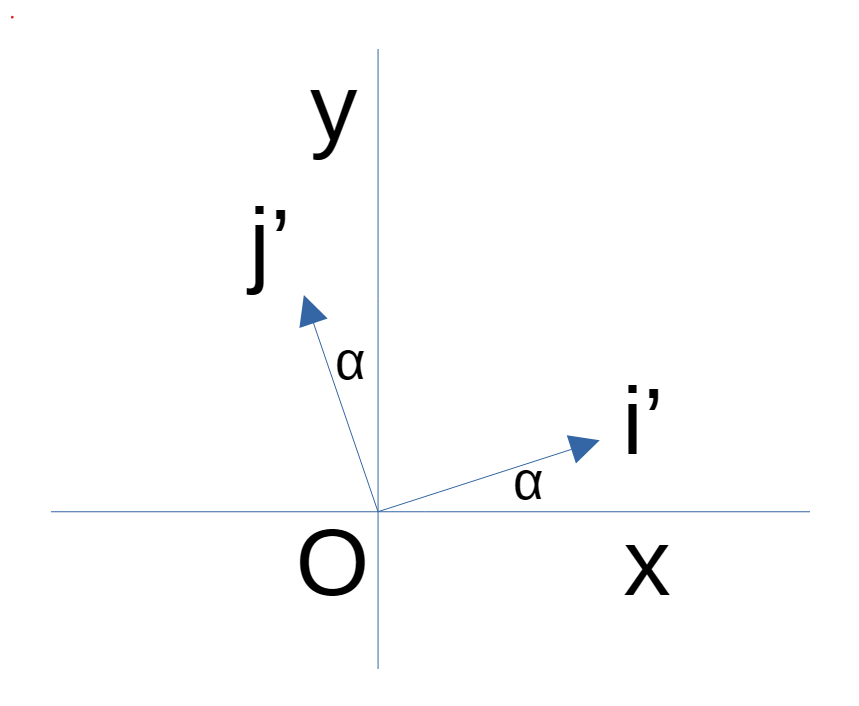
\includegraphics[width=0.7\textwidth]{rotation_alpha_007.png}
%==========================================
\end{center}

\caption{\label{kn:versor_rotation_alpha}
Obracamy układ współrzędnych $Oxy$ o kąt $\alpha$ przeciwnie do ruchu wskazówek zegara 
wokół osi $Oz$
otrzymując
układ współrzędnych $Ox'y'$\@. Oznacza to, że wersory $i$ oraz $j$
zostają obrócone 
o kąt $\alpha$ i przechodzą w wersory $i'$ oraz $j'$\@. Na rysunku oznaczenia wersorów $i$ oraz $j$ 
na osiach $Ox$ i $Oy$ dla przejrzystości pominięto.}
\end{figure}

Składając obrót wersorów $i$ oraz $j$ o kąt $\alpha$ z obrotem o kąt $\beta$ otrzymujemy macierz obrotu tych wersorów o kąt $\alpha + \beta$\@.
Z odpowiednich podstawień otrzymujemy następujące wzory trygonometryczne
\begin{equation}
\sin(\alpha + \beta) = \sin \alpha \cos \beta + \cos \alpha \sin \beta
\end{equation}
\begin{equation}
\cos(\alpha + \beta) = \cos \alpha \cos \beta - \sin \alpha \sin \beta
\end{equation}



\section{Obrót wektora}\label{sec2}

Niech będzie dany wektor $\vec{r}$ tworzący kąt $\theta$ z osią $Ox$
\begin{equation}
\vec{r} = x \, i + y \, j = r \cos \theta \, i + r \sin \theta \, j 
\end{equation}
Obracając ten wektor $\vec{r}$ o kąt $\alpha$ 
otrzymamy wektor $\vec{r}^{\,\,'}$ tworzący kąt $\theta + \alpha$ z osią $Ox$
\begin{equation}
\vec{r}^{\,\,'} = r \cos( \theta + \alpha ) \, i + r \sin( \theta + \alpha ) \, j
\end{equation}
\begin{eqnarray}
\vec{r}^{\,\,'} = r (\cos \theta \cos \alpha - \sin \theta \sin \alpha) \, i
+                 r (\sin \theta \cos \alpha + \cos \theta \sin \alpha) \, j         =  \\ \nonumber
=
( r \cos \theta \cos \alpha - r \sin \theta \sin \alpha ) \, i 
+
( r \sin \theta \cos \alpha + r \cos \theta \sin \alpha ) \, j                       =  \\ \nonumber
=
( x \cos \alpha - y \sin \alpha ) \, i 
+
( y \cos \alpha + x \sin \alpha ) \, j 
\end{eqnarray}
Z powyższego otrzymujemy, że współrzędne $x'$ oraz $y'$ wektora $\vec{r}$ obróconego o kąt $\alpha$  wynoszą
\begin{eqnarray}
x' = x \cos \alpha - y \sin \alpha      \\ 
y' = x \sin \alpha + y \cos \alpha
\end{eqnarray}
co w zapisie macierzowym daje
\begin{equation}
\begin{bmatrix}
x' \\ 
y' 
\end{bmatrix}
=
\begin{bmatrix*}[r]
 \cos \alpha  & -\sin \alpha  \\
 \sin \alpha  &  \cos \alpha
\end{bmatrix*}
\begin{bmatrix}
x \\ 
y 
\end{bmatrix}
\end{equation}



\section{Mnożenie macierzy}\label{sec3}


Jeżeli chcielibyśmy obrócić wektor o współrzędnych $x, y$ najpierw o kąt $\alpha$ a następnie o kąt $\beta$
wokół osi $Oz$ to musielibyśmy złożyć dwa obroty co odpowiada w macierzowym zapisie
\begin{equation}
\begin{bmatrix}
x'' \\ 
y'' 
\end{bmatrix}
=
\begin{bmatrix*}[r]
 \cos \beta  & -\sin \beta  \\
 \sin \beta  &  \cos \beta
\end{bmatrix*}
\begin{bmatrix*}[r]
 \cos \alpha  & -\sin \alpha  \\
 \sin \alpha  &  \cos \alpha
\end{bmatrix*}
\begin{bmatrix}
x \\ 
y 
\end{bmatrix}
\end{equation}
a skrótowo
\begin{equation}
\mathbf{r}'' =    \mathbf{B} \mathbf{A} \mathbf{r}
\end{equation}
gdzie
\begin{equation}
\mathbf{A}
=
\begin{bmatrix*}[r]
 \cos \alpha  & -\sin \alpha  \\
 \sin \alpha  &  \cos \alpha
\end{bmatrix*}
\hspace{1.0cm}
\mathbf{B}
=
\begin{bmatrix*}[r]
 \cos \beta  & -\sin \beta  \\
 \sin \beta  &  \cos \beta
\end{bmatrix*}
\end{equation}

Jeżeli wyliczymy $x'$ oraz $y'$
z operacji macierzowej
\begin{equation}
\mathbf{r}' =    \mathbf{A} \mathbf{r}
\end{equation}
a następnie $x''$ oraz $y''$
\begin{equation}
\mathbf{r}'' =    \mathbf{B} \mathbf{r}'
\end{equation}
to okaże się, że wynik jaki otrzymamy jest równoważny mnożeniu
\begin{equation}
\mathbf{r}'' =    \mathbf{C} \mathbf{r}
\end{equation}
gdzie
\begin{equation}
\mathbf{C} = \mathbf{B} \mathbf{A}
\end{equation}
przy czym wyrazy $c_{m,n}$ macierzy $\mathbf{C}$ są wyliczone jako
\begin{equation}
c_{m,n} = \sum_{k} b_{m,k} a_{k,n}
\end{equation}
Zapis $c_{m,n}$ odnosi się do elementu macierzy $\mathbf{C}$ w $m$-tym wierszu oraz w $n$-tej kolumnie.
Można się przekonać o tym podstawiając odpowiednie wartości elementów macierzy obrotów
do równania na $\mathbf{r}$, $\mathbf{r}'$ oraz na $\mathbf{r}''$ gdzie
\begin{equation}
\mathbf{r} =
\begin{bmatrix}
x \\ 
y 
\end{bmatrix} \hspace{1.0cm}
\mathbf{r}' =
\begin{bmatrix}
x' \\ 
y' 
\end{bmatrix} \hspace{1.0cm}
\mathbf{r}'' =
\begin{bmatrix}
x'' \\ 
y'' 
\end{bmatrix}
\end{equation}

Zauważamy, że jeżeli $\mathbf{A}$ jest macierzą obrotu o kąt $\alpha$
oraz $\mathbf{B}$ jest macierzą obrotu o kąt $\beta$ a obie rotacje są wokół osi $Oz$ to wtedy mamy
\begin{equation}
\mathbf{B} \mathbf{A} = \mathbf{A} \mathbf{B}
\end{equation}
ponieważ kolejność obrotów wokół tej samej osi nie ma znaczenia i najpierw możemy dokonać obrotu o kąt $\alpha$
a potem o kąt $\beta$ lub w odwrotnym porządku a otrzymamy ten sam rezultat złożenia obrotów.
W przypadku takich obrotów mnożenie macierzowe jest przemienne jednakże w ogólności mnożenie macierzowe macierzy 
$\mathbf{A}$ i $\mathbf{B}$
przemienne nie jest
\begin{equation}
\mathbf{A} \mathbf{B} \neq \mathbf{B} \mathbf{A}
\end{equation}




\end{document}

%%%%%%%%%%%%%%%%%%%%%%%%%%%%%%%%%%%%%%%%%%%%%%%%%%%%%%%%%%%%%%%


\section{Mnożenie macierzy}\label{sec3}


In the equation
\begin{eqnarray}
\label{eq:matrix_equation_for_coordinates_of_rotated_vector}
  \begin{bmatrix}
    v_{x}' \\
    v_{y}'
  \end{bmatrix}
=
  \begin{bmatrix}
    \cos \alpha & -\sin \alpha \\
    \sin \alpha &  \cos \alpha
  \end{bmatrix}
  \begin{bmatrix}
    v_{x} \\
    v_{y}
  \end{bmatrix}
\end{eqnarray}
the expression
\begin{eqnarray}
\label{eq:matrix_for_coordinates_of_rotated_vector}
  \begin{bmatrix}
    \cos \alpha & -\sin \alpha \\
    \sin \alpha &  \cos \alpha
  \end{bmatrix}
\end{eqnarray}
is called the matrix of rotation of the vector
\begin{eqnarray}
\label{eq:original_vector}
  \begin{bmatrix}
    v_{x} \\
    v_{y}
  \end{bmatrix}
\end{eqnarray}
by angle $\alpha$ about the $Oz$ axis counterclockwise.
Rotated vector has the coordinates
\begin{eqnarray}
\label{eq:rotated_vector}
  \begin{bmatrix}
    v_{x}' \\
    v_{y}'
  \end{bmatrix}
\end{eqnarray}
which are computed as
\begin{eqnarray}
\label{eq:rotated_vector_coordinates_expression}
v_{x}' = v_{x} \cos \alpha - v_{y} \sin \alpha    \\ \nonumber
v_{y}' = v_{x} \sin \alpha + v_{y} \cos \alpha    
\end{eqnarray}
Equations~(\ref{eq:matrix_equation_for_coordinates_of_rotated_vector})
and~(\ref{eq:rotated_vector_coordinates_expression}) are equivalent.
The expressions in equations~(\ref{eq:rotated_vector_coordinates_expression})
are just the results of multiplication of the vector~(\ref{eq:original_vector})
by the matrix~(\ref{eq:matrix_for_coordinates_of_rotated_vector})\@.
As the result of such multiplication of the vector~(\ref{eq:original_vector})
by the matrix~(\ref{eq:matrix_for_coordinates_of_rotated_vector})
we receive a column vector~(\ref{eq:column_vector_of_results_of_matrix_multiplication})
\begin{eqnarray}
\label{eq:column_vector_of_results_of_matrix_multiplication}
  \begin{bmatrix}
    v_{x} \cos \alpha - v_{y} \sin \alpha \\
    v_{x} \sin \alpha + v_{y} \cos \alpha
  \end{bmatrix}
\end{eqnarray}
The column vector~(\ref{eq:column_vector_of_results_of_matrix_multiplication}) has the coordinates
of the vector~(\ref{eq:original_vector}) which is rotated counterclockwise by
the angle $\alpha$ around the $Oz$ axis.


Let us now apply the matrix of counterclockwise rotation 
around the axis $Oz$
by the angle $\beta$ on the coordinates
of the column vector~(\ref{eq:column_vector_of_results_of_matrix_multiplication})

\begin{eqnarray}
\label{eq:matrix_equation_for_coordinates_of_twice_rotated_vector}
  \begin{bmatrix}
    v_{x}'' \\
    v_{y}''
  \end{bmatrix} 
=
  \begin{bmatrix}
    \cos \beta & -\sin \beta \\
    \sin \beta &  \cos \beta
  \end{bmatrix}
  \begin{bmatrix}
    v_{x}' \\
    v_{y}'               
  \end{bmatrix}
  =
  \begin{bmatrix}
    \cos \beta v_{x}'  - \sin \beta v_{y}'  \\
    \sin \beta v_{x}'  + \cos \beta v_{y}'
  \end{bmatrix}
=                                                 \\ \nonumber
=
  \begin{bmatrix}
    \cos \beta (v_{x} \cos \alpha - v_{y} \sin \alpha)  - \sin \beta (v_{x} \sin \alpha + v_{y} \cos \alpha)  \\
    \sin \beta (v_{x} \cos \alpha - v_{y} \sin \alpha)  + \cos \beta (v_{x} \sin \alpha + v_{y} \cos \alpha)
  \end{bmatrix}                                                                                               \\ \nonumber
=
  \begin{bmatrix}
  v_{x}(\cos \alpha \cos \beta - \sin \alpha \sin \beta) - v_{y}(\sin \alpha \cos \beta + \cos \alpha \sin \beta) \\
  v_{x}(\sin \alpha \cos \beta + \cos \alpha \sin \beta) + v_{y}(\cos \alpha \cos \beta - \sin \alpha \sin \beta)
  \end{bmatrix}                                                                                                   \\ \nonumber
  =
 \begin{bmatrix}
  \cos \alpha \cos \beta - \sin \alpha \sin \beta & -(\sin \alpha \cos \beta + \cos \alpha \sin \beta) \\
  \sin \alpha \cos \beta + \cos \alpha \sin \beta &   \cos \alpha \cos \beta - \sin \alpha \sin \beta
 \end{bmatrix}  
   \begin{bmatrix}
    v_{x} \\
    v_{y}               
  \end{bmatrix}                                                                                                \\ \nonumber
  =
    \begin{bmatrix}
    \cos \beta & -\sin \beta \\
    \sin \beta &  \cos \beta
  \end{bmatrix}
    \begin{bmatrix}
    \cos \alpha & -\sin \alpha \\
    \sin \alpha &  \cos \alpha
  \end{bmatrix}
    \begin{bmatrix}
    v_{x} \\
    v_{y}               
  \end{bmatrix} 
  % \begin{bmatrix}
  %   \cos \beta & -\sin \beta \\
  %   \sin \beta &  \cos \beta
  % \end{bmatrix}
  %   \begin{bmatrix}
  %   v_{x} \cos \alpha - v_{y} \sin \alpha \\
  %   v_{x} \sin \alpha + v_{y} \cos \alpha
  % \end{bmatrix}
\end{eqnarray}

We can write
\begin{eqnarray}
\label{eq:matrix_multiplication_for_matrices_of_rotatation}
    \begin{bmatrix}
    \cos \beta & -\sin \beta \\
    \sin \beta &  \cos \beta
  \end{bmatrix}
    \begin{bmatrix}
    \cos \alpha & -\sin \alpha \\
    \sin \alpha &  \cos \alpha
  \end{bmatrix}                                                                                \\ \nonumber
=
 \begin{bmatrix}
  \cos \alpha \cos \beta - \sin \alpha \sin \beta & -( \sin \alpha \cos \beta + \cos \alpha \sin \beta ) \\
  \sin \alpha \cos \beta + \cos \alpha \sin \beta &  \cos \alpha \cos \beta - \sin \alpha \sin \beta
 \end{bmatrix}                                                                                  \\ \nonumber
=
    \begin{bmatrix}
    \cos (\alpha + \beta) & -\sin (\alpha + \beta) \\
    \sin (\alpha + \beta) &  \cos (\alpha + \beta)
  \end{bmatrix} 
\end{eqnarray}
By comparison from equation~(\ref{eq:matrix_multiplication_for_matrices_of_rotatation})
we see that we receive the formulas for $\cos (\alpha + \beta)$ and $\sin (\alpha + \beta)$ as
\begin{equation}
\cos (\alpha + \beta) = \cos \alpha \cos \beta - \sin \alpha \sin \beta
\end{equation}
\begin{equation}
\sin (\alpha + \beta) = \sin \alpha \cos \beta + \cos \alpha \sin \beta
\end{equation}
If we write
\begin{eqnarray}
\label{eq:matrix_A}
A
=
  \begin{bmatrix}
    \cos \alpha & -\sin \alpha \\
    \sin \alpha &  \cos \alpha
  \end{bmatrix}
\end{eqnarray}
and
\begin{eqnarray}
\label{eq:matrix_B}
B
=
  \begin{bmatrix}
    \cos \beta & -\sin \beta \\
    \sin \beta &  \cos \beta
  \end{bmatrix}
\end{eqnarray}
we can compute the product of matrices $BA = C$
\begin{eqnarray}
\label{eq:matrix_C}
C
=
 \begin{bmatrix}
  \cos \alpha \cos \beta - \sin \alpha \sin \beta & -( \sin \alpha \cos \beta + \cos \alpha \sin \beta ) \\
  \sin \alpha \cos \beta + \cos \alpha \sin \beta &    \cos \alpha \cos \beta - \sin \alpha \sin \beta
 \end{bmatrix}  
\end{eqnarray}
We notice that if   $a_{i,j}, b_{i,j}, c_{i,j}$ denote the matrix element from $i$-th row and $j$-th column
from the matrix $A, B, C$, respectively, we may write
\begin{eqnarray}
\label{eq:matrix_A_ij}
A
=
 \begin{bmatrix}
  a_{1,1} &  a_{1,2} \\
  a_{2,1} &  a_{2,2}
 \end{bmatrix}  
\end{eqnarray}
\begin{eqnarray}
\label{eq:matrix_B_ij}
B
=
 \begin{bmatrix}
  b_{1,1} &  b_{1,2} \\
  b_{2,1} &  b_{2,2}
 \end{bmatrix}  
\end{eqnarray}
and
\begin{eqnarray}
\label{eq:matrix_C_ij}
C
=
 \begin{bmatrix}
  c_{1,1} &  c_{1,2} \\
  c_{2,1} &  c_{2,2}
 \end{bmatrix}  
\end{eqnarray}
and
we have for the matrix multiplication of the matrices $AB$ equals $C$
when A, B have the dimensions two rows by two columns
\begin{eqnarray}
\label{eq:matrix_B_times_A_equals_C}
 % \begin{bmatrix}
c_{i,j} = a_{i,1} b_{1,j}  +   a_{i,2} b_{2,j}
 % \end{bmatrix}  
\end{eqnarray}
In general for the matrices of dimensions $N$ by $N$ we have
\begin{eqnarray}
\label{eq:matrix_B_times_A_equals_C_dimensions_N_by_N}
 % \begin{bmatrix}
c_{i,j} = \sum_{k = 1}^{N} a_{i,k} b_{k,j} 
 % \end{bmatrix}  
\end{eqnarray}
We notice that when $A$ is the rotation matrix by the angle $\alpha$
and $B$ is the rotation matrix by the angle $\beta$, both rotations around the $Oz$ axis, we have
\begin{equation}
AB = BA
\end{equation}
because the order of rotations does not matter, and first we may rotate by the angle $\alpha$
then by the angle $\beta$ or in the reversed order and we will receive the same result of rotations.
In case of such rotations the matrix multiplication is commutative
however the matrix multiplication is not commutative in general and for any matrices
$A$, $B$
\begin{equation}
AB \neq BA
\end{equation}





\end{document}
